\documentclass[12pt, a4paper]{article}

% --- Pacotes Básicos ---
\usepackage[utf8]{inputenc}
\usepackage[]{graphicx}
\usepackage[T1]{fontenc}
\usepackage{times}
\usepackage{setspace}
\onehalfspacing % Set line spacing to 1.5
\setlength{\parindent}{1.25cm}
\setlength{\lineskip}{1.5cm}
%\usepackage[main=brazilian, english]{babel}
\usepackage{indentfirst}
\usepackage{geometry}
\geometry{left=3cm, top=3cm, right=2cm, bottom=2cm}

\usepackage{etoolbox} % Pacote necessário para ajustar o espaçamento

% Criando o ambiente 'citacao'
\newenvironment{citacao}{
  \vspace{0.5cm} % Espaço antes da citação
  \small % Letra menor (geralmente tamanho 10)
  \begin{list}{}{
    \leftmargin=4cm % Recuo de 4 cm da margem esquerda
    \rightmargin=0cm
    \parsep=0pt
    \topsep=0pt
    \partopsep=0pt
  }
  \item\relax
  \linespread{1.0}\selectfont % Garante espaçamento simples dentro da citação
}{
  \end{list}
  \vspace{0.5cm} % Espaço depois da citação
}
% --- Informações do Documento ---
\title{UNIVERSIDADE FEDERAL DA FRONTEIRA SUL\\Ciência da Computação\\História da Fronteira Sul\\Prof. Fernando Vojniak\\Continuidade e mudança do território Kaingang do Rio Grande do Sul: um estudo de caso do aldeamento de Nonoai}
\date{}

\begin{document}
\maketitle

\begin{flushright}
	Erickson Giesel Muller
\end{flushright}

	CURTA, Jussara Costa. \textbf{Continuidade e mudança do território Kaingang do Rio Grande do Sul: um estudo de caso do aldeamento de Nonoai}. 2012.
	\\
\thispagestyle{empty} % primeira página não tem número.

	O texto intitulado \textit{Continuidade e Mudança do Território Kaingang do Rio Grande do Sul: Um Estudo de Caso do Aldeamento de Nonoai} é Trabalho de Conclusão de Curso em História escrito por Jussara Costa Curta da Universidade Federal do Rio Grande do Sul (UFRGS). Defendido em 2012 sob a orientação da Profa. Dra. Adriana Schmidt Dias, doutora em arqueologia pela Universidade de São Paulo (USP), atualmente é professora titular do Departamento de História da UFRGS. O objetivo do estudo é a naálise do processo de expropriação das terras tradicionais Kaingang na Província do Rio Grande do Sul, sobretudo no período de 1848 a 1889, com a institucionalização da Lei de Terras. A pesquisa busca compreender as concepções de territorialidade e identificar estratégias de resistência e negociação utilizadas pelos nativos para a manutenção de seu espaço, usando como objeto de estudo o aldeamento de Nonoai.

A limitação temporal é dada para investigar o processo de expropriação do território nativo Kaingang e analisar as diferentes estratégias, tanto de resistência quanto de negociação, mobilizadas pelos indígenas para a manutenção de suas terras tradicionais. A escolha pelo aldeamento de Nonoai justifica-se pelo fato de este ser um dos territórios em que os povos indígenas promoveram mais ações e reações frente à expropriação territorial, permitindo compreender a organização indígena e sua resistência diante do contexto histórico.

A autora cita que a filiação linguística dos Kaingang ao Tronco Macro-Jê e à Família Jê revela uma trajetória histórica que remonta originalmente ao Brasil Central, em áreas localizadas entre as bacias dos rios São Francisco, Araguaia e Tocantins (pg. 8). De acordo com modelos de reconstrução linguística, esse grupo teria se separado de outros povos Jê há cerca de 3 mil anos, iniciando um longo processo migratório rumo ao sul do continente. Essa movimentação não foi aleatória, os grupos buscaram regiões de planalto no Sul do Brasil devido à semelhança com o seu seu habitat de origem, permitindo assim a manutenção de padrões de adaptação e subsistência já consolidados.

A arqueologia fundamenta a tese da continuidade histórica dos Kaingang através da chamada "Tradição Taquara", identificada pelos arqueológicos pela presença de pequenos vasos cerâmicos e estruturas de terra. O elemento mais emblemático dessa tradição são as "casas subterrâneas", moradias escavadas em regiões de altitude acima de 500 metros que serviam como uma proteção engenhosa contra os invernos rigorosos do Planalto Meridional. As pesquisas demonstram que as áreas dessas ocupações pré-históricas, que remontam ao século II d.C., coincidem geograficamente com os territórios ocupados pelos Kaingang em períodos posteriores, comprovando raízes culturais milenares na região (p. 23).

O texto descreve que a ocupação histórica dos Kaingang no sul do Brasil demonstra uma relação de profunda integração com o meio ambiente, coincidindo com a distribuição das florestas de araucária (p. 13). Essa matas eram essenciais para a subsistência do grupo nesse período, mas também para seu sedentarismo, dado que o pinhão é um recurso alimentar que serviatanto para a nutrição imediata quanto para provisões em estações de escassez. O ambiente florestal das terras altas oferecia proteção contra o clima frio e os fortes ventos da região, influenciando inclusive o modelo de construção das moradias do grupo. O valor desses pinheirais era tão expressivo para a população indígena que esse recurso era rigorosamente dividido entre as tribos, com limites demarcados nas cascas dos pinheiros através de marcas e pinturas que refletiam a identidade social dos ocupantes da área (p. 19).

\begin{center}
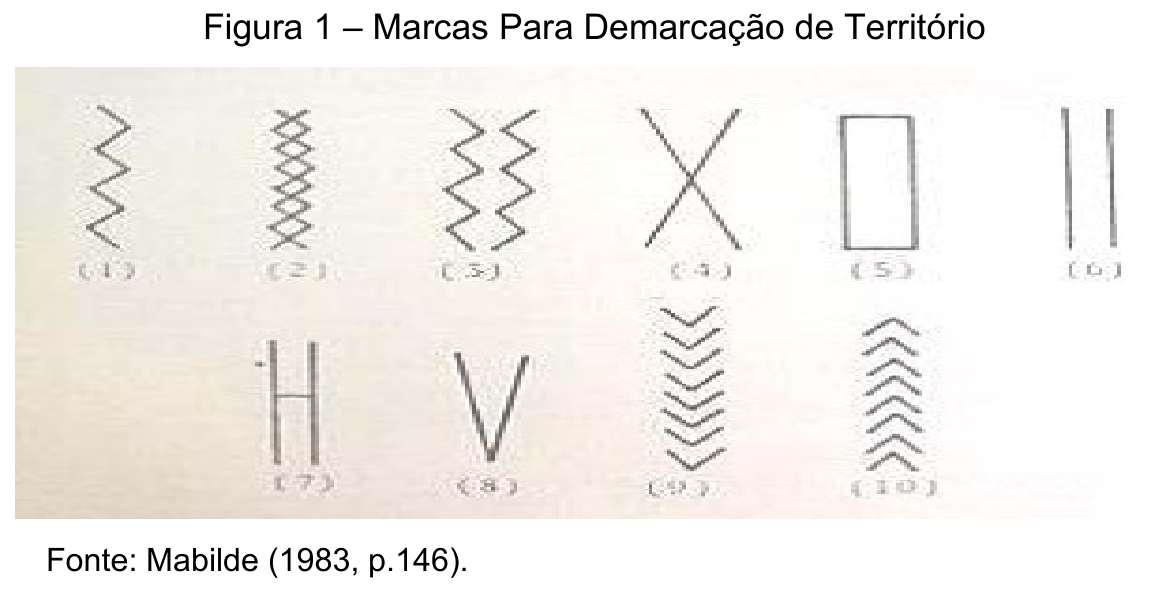
\includegraphics[scale=0.4]{images/pinheiros.png}
\end{center}

As denominações atribuídas aos grupos Jê Meridionais eram variadas e, inicialmente, apelidadas a partir de colonizadores. Historicamente, foram identificados pelo historiador Pedro Lozano como "Guaianá" (p. 16), termo que englobava diversas tribos com costumes e línguas distintos dos Guarani. Entretanto, até meados do século XIX, a denominação que se tornou generalizada na Província do Rio Grande do Sul e em outras partes do Império foi a de "Coroados". \textbf{De acordo com os registros do engenheiro Alphonse Mabilde(1983)}, esse nome derivava do costume desses indígenas de tonsurarem seus cabelos. O termo "Kaingang" só começou a surgir na bibliografia a partir de 1882, sendo consolidado posteriormente como uma designação genérica para os diversos grupos de dialetos aparentados e filiados ao tronco linguístico Jê.

A estrutura política dos Kaingang no século XIX era organizada em pequenas tribos compostas por núcleos familiares e parentes próximos. Cada uma dessas unidades possuía seu próprio cacique local que respondia hierarquicamente a um cacique principal. Este cacique central exercia autoridade direta sobre a gestão de todo o territorio território, sendo responsável por indicar o local específico que cada tribo subordinada deveria habitar. A estabilidade dessas relações dependia de um complexo sistema de visitas periódicas de caráter político; quando uma guerra era declarada entre as tribos, essas visitas eram suspensas por ordem do cacique principal. A autora pontua que eram frequentes os conflitos entre os indígenas dessa região, envolvendo tanto dissidências internas quanto disputas territoriais contra grupos rivais de outras etnias, como os Xokleng e os Guarani.

Os ciclos da natureza determinaram o modo de subsistência dos Kaingang do século XIX, marcada pela exploração de diferentes ecossistemas. A agricultura era praticada em terrenos elevados, onde se cultivavam diversas variedades de milho, feijão, abóbora e amendoim. A coleta desempenhava um papel central na dieta e na cultura, com destaque absoluto para o pinhão, o alimento mais prestigiado e cuja exploração seguia regras rígidas de propriedade territorial (p. 19). Além do pinhão, o grupo coletava mel, palmito, corós, raízes e uma grande variedade de frutos sazonais, como o araçá, a pitanga e a guabiroba. A obtenção de proteína animal acontecia principalmente pela caça de espécies como a anta, o porco, o tatu e a paca, além da pesca realizada durante os meses de verão em locais mais afastados das aldeias.

É possível perceber como a autora, reiteradamente, lembra o leitor que a noção de propriedade dos povos originários se afasta da noção hegemônica ocidental.
\begin{citacao}
	Para as comunidades indígenas, a terra representa muito mais do que um  simples meio de subsistência. É o elemento essencial, pois representa o suporte da  vida social e está diretamente ligada ao sistema de crenças e conhecimento. Logo, a  terra não é apenas um recurso natural, mas está diretamente ligada ao cotidiano  como um todo interligado, representando a base da vida sociocultural (RAMOS, 1988, pg. 23)
\end{citacao}
Essa concepção de territorialidade caracteriza consideravelmente sua cultura, na qual a ligação com a "terra-mãe" é estabelecida desde o nascimento até a morte. O território é, portanto, um espaço carregado de conteúdo simbólico e histórico, estruturado por explicações míticas fundamentais, como a do grande dilúvio, no qual os antepassados Kaingang sobreviveram ao buscar o cume da serra Krinjijimbé (Serra do Mar), que sobressaía das águas. Diferente da visão puramente geográfica e utilitária da sociedade nacional do período, para o indígena a relação com o território tradicional é vital para a afirmação de sua identidade étnica.

Não se confunde a noção que os Kaingang tinham sobre a propriedade territorial com o conceito capitalista de propriedade privada, aqueles tiveram grande influência das suas relações sociais e pelo direito de uso coletivo do território. Ter uma propriedade comum do solo não siginificava uma ausência de normas, pelo contrário, existiam direitos precisos e definidos que regulavam o acesso ao espaço. A divisão dos pinheirais entre as tribos foi um sistema de direitos comunitários que assegurava que todos os membros tivessem acesso aos recursos fundamentais, garantindo que as gerações futuras recebessem a herança desse território.

O texto descreve como o Estado utilizou de mitos historiográficos para legitimar o deslocamento dos povos indígenas, especialmente as noções de "nomadismo" e de "vazio demográfico". O nomadismo foi usado de argumento para justificar a expropriação de terras e a destituição do direito dos nativos sobre o solo. Também o vazio demográfico é apresentado como um discurso oficial que visava ocultar a presença indígena, tratando as terras do planalto como "devolutas" ou desabilitadas para viabilizar uma ocupação produtiva pela lógica dos colonizadores. O estudo critica esse mitos, argumentando que os Kaingang já eram agricultores antes do contato com os europeus e que o Estado Provincial ignorou as evidências arqueológicas de ocupação milenar (pg. 26-27).

A Lei de Terras de 1850 institucionalizou a exclusão das comunidades indígenas ao estabelecer novos princípios para a ocupação do solo que favoreciam a mercantilização da terra. A lei exigia a comprovação de "morada habitual" e "cultura efetiva" para a legitimação das posses, parâmetros que ignoravam a lógica territorial da sociedade nativa (pg. 31). Como as atividades fundamentais dos Kaingang como a caça, a pesca, a coleta sazonal e a mobilidade geográfica não se enquadravam nas exigências de vida sedentária e agricultura permanente da nova lei, seus roçados e habitações tradicionais não foram considerados ocupações legítimas. Essas terras, consideradas agora "devolutas", foram disponibilizadas pelo Estado para a expansão do latifúndio e projetos de colonização europeia, criando um conflito dos indígenas pela defesa de seu território ancestral (pg. 31).


O aldeamento de Nonoai, localizado no extremo noroeste do Rio Grande do Sul, foi fundado em 1848 e posteriormente ratificado pela Lei de Terras. Sua criação foi resultado de uma política provincial que buscava concentrar as populações indígenas em áreas reduzidas, bucando minimizar contatos violentos e garantir mais segurança para a ocupação colonial. Essa política possibilitou aos colonos, principalmente alemães e italianos, estabelecer municípios na região. O aldeamento facilitava o desenvolvimento de infraestruturas, como a abertura de estradas ligando as Províncias do Rio Grande e de São Paulo (pg. 33). Com esse apontamento, a autora explicita como a migração e estabelecimento indígena para a região foi fruto de decisões políticas do governo imperial.

O início do aldeamento de Nonoai foi permeado por conflitos e invasões territoriais. Um caso notório de abuso de poder foi o de Cipriano Rocha de Loures, o primeiro diretor do núcleo, que aproveitou sua posição para cercar três léguas das terras massi férteis do aldeamento em benefício próprio. Loures foi descrito como um grande manipulador, utilizando de ameaças de perseguição armada para forçar a saída dos nativos, chegando a destuir suas habitações para garantir a posse dos campos (pg. 38). Concomitantemente, o avanço de posseiros como Clementino Pacheco, que se apoderou de terras reclamadas pelos indígenas sem que o governo tomasse as devidas providências, gerou hostilidades que resultaram em tragédias. A resistência Kaingang manifestou-se de forma violenta quando o índio Pedro Nicofim matou Pacheco e outras cinco pessoas, evidenciando que o grupo reagia com vigor contra a expropriação de seus territórios sagrados e de seus meios de subsistência (pg. 39).

As táticas para garantir a manutenção do território Kaingang foi personificada por figuras de lideranças como os caciques Nonoai, Doble e Condá. O Cacique Nonoai destacou-se por sua liderança histórica na defesa das terras de seus antepassados, legitimando a posse dos campos por meio de vínculos de nascimento e ancestralidade. Simultaneamente, líderes como Vitorino Condá e Doble adotaram estratégias de colaboracionismo, atuando como mediadores e batedores junto às autoridades provinciais e colonizadores em troca de segurança, alimentos e gratificações para seus grupos. O estudo cita o caráter ambíguo de Cacique Doble, ao mesmo tempo que colaborava com o governo na captura de grupos "arredios", participava de "correrias" (ataques violentos contra fazendas e lotes coloniais) para resistir à expropriação de suas áreas de caça e coleta (pg. 42). Dessa forma, a ação indígena se manifestou na capacidade de alternar entre a diplomacia e o uso da força física, transformando o aldeamento em um espaço de negociação e resistência estratégica frente às pressões da colonização expansionista.

O estudo conclui que os Kaingang não foram passivos frente à perda de suas terras, mas sim sujeitos ativos que desenvolveram lógicas e comportamentos próprios em reação às adversidades impostas pela colonização e expansão da sociedade nacional. Dentro da estrutura dos aldeamentos, esses grupos reelaboraram estratégias de sobrevivência, utilizando seus espaços não apenas como locais de assentamento, mas como uma forma tática de manter parte de seu território original e estabelecer um campo necessário de negociação com a sociedade envolvente para garantir sua existência física e cultural. A resistência indígena manifestou-se por meio de ações diversificadas e complexas, que incluíram desde alianças estratégicas e colaboracionismo com autoridades provinciais até atos de resistência direta e violenta, demonstrando que os Kaingang lutaram ativamente pela preservação de seus interesses e terras tradicionais. Essa postura histórica de protagonismo fundamenta a relevância atual do grupo, que hoje continua mobilizando a concepção tradicional de território para lutar pela demarcação e recuperação de suas terras ancestrais.

O texto representa bem como este povo permanece como o grupo indígena mais numeroso do Sul do Brasil e a maior representação da família linguística Macro-Jê. Com uma população estimada em aproximadamente 29 mil indivíduos distribuídos por dezenas de áreas entre São Paulo e o Rio Grande do Sul, o grupo transformou sua resiliência demográfica em um motor para novas reivindicações. Percebe-se como o estudo contraria a noção comum acrítica de que os povos originários foram agentes passivos da imposição colonizadora e demonstra com exemplos como esses povos tiveram ações de resistência e negociação que foram determinantes para sua história. Nesse contexto, os Kaingang buscam intensificar alianças institucionais e sociais para garantir a demarcação de espaços tradicionais ainda disponíveis, utilizando argumentos que unem a memória dos antepassados aos seus próprios significados socio-cosmológicos. Recomenda-se também a leitura de textos citados no trabalho da autora.

%\begin{thebibliography}{99}
%
%\bibitem{curta2012}
%
%\bibitem{mabilde1983} 
%	MABILDE, Pierre F. A. B. \textbf{Apontamentos sobre os indígenas selvagens da Nação Coroados das matas da Província do Rio Grande do Sul}: 1836-1866. São Paulo: IBRASA, Fundação Nacional Pró-Memória, 1983.
%
%\bibitem{prous1992}
%	PROUS, André. \textbf{Arqueologia Brasileira}. Brasília: Editora da UnB, 1992.
%
%\bibitem{tommasino1995}
%	TOMMASINO,  Kimiye.  \textbf{A  História  dos  Kaingáng  da  Bacia  do  Tibagi:  Uma  Sociedade Jê Meridional em Movimento}. São Paulo: USP, 1995. Tese (Doutorado  em Antropologia) – Instituto de Filosofia e Ciências Humanas, Universidade de São  Paulo, 1995. 
%\end{thebibliography}
%
\end{document}
